\documentclass[11pt,aspectratio=169]{beamer}
\usepackage{fontspec}
\usepackage{amsmath,amssymb}
\usepackage{microtype}
\usepackage{booktabs}
\graphicspath{{figs/}{../../figures/exp1/}}

% palette: dove base + dark overrides
\usecolortheme{dove}
\colorlet{mut}{white!52!black}
\colorlet{acc}{cyan!55!white}
\setbeamercolor{background canvas}{bg=black}
\setbeamercolor{normal text}{fg=white,bg=black}
\setbeamercolor{structure}{fg=white}
\setbeamercolor{frametitle}{fg=white}
\setbeamercolor{title}{fg=white}
\setbeamercolor{subtitle}{fg=mut}
\setbeamercolor{author}{fg=mut}
\setbeamercolor{date}{fg=mut}
\setbeamercolor{alerted text}{fg=acc}
\setbeamercolor{itemize item}{fg=mut}
\setbeamercolor{itemize subitem}{fg=mut}

\setbeamertemplate{navigation symbols}{}
\setbeamertemplate{itemize item}{\small\raise0.15ex\hbox{\textbullet}}
\setbeamertemplate{itemize subitem}{\scriptsize\raise0.15ex\hbox{--}}
\setbeamerfont{frametitle}{size=\large,series=\bfseries}
\setbeamerfont{title}{size=\Large,series=\bfseries}

% frame title + hairline rule underneath
\setbeamertemplate{frametitle}{%
  \vspace{0.8em}%
  {\usebeamerfont{frametitle}\usebeamercolor[fg]{frametitle}\insertframetitle\par}%
  \vspace{0.25em}{\color{mut!45}\hrule height 0.4pt}\vspace{-0.2em}%
}
% muted footer: short title (left) + frame number (right)
\setbeamertemplate{footline}{%
  \hbox{\begin{beamercolorbox}[wd=\paperwidth,ht=2.4ex,dp=1.4ex,leftskip=1.2em,rightskip=1.2em]{}%
    {\color{mut}\scriptsize \insertshorttitle}\hfill{\color{mut}\scriptsize\insertframenumber}%
  \end{beamercolorbox}}%
}
\setbeamertemplate{title page}{%
  \vfill{\usebeamerfont{title}\usebeamercolor[fg]{title}\inserttitle\par}
  \vspace{0.6em}{\color{mut}\normalsize\insertsubtitle\par}
  \vspace{1.6em}{\color{mut}\small\insertauthor\par}
  \vspace{0.3em}{\color{mut}\footnotesize\insertdate\par}\vfill
}

\title[PE metadata drift: Experiment 1 progress]{Which Metadata Can the PE Vote See?}
\subtitle{Experiment 1 results and a re-annotation plan}
\author{Kando Hsieh \quad\textbullet\quad Eli Lab}
\date{October 13, 2026}

\begin{document}

\begin{frame}[plain]\titlepage\end{frame}

% ------------------------------------------------------------------ 2
\begin{frame}{Two scores per attribute: what the vote can use vs.\ what $\phi$ encodes}
$\phi$ = sentence-t5-base, the embedding of MAPLE's $L_2$ 1-NN vote. bioRxiv, $9$ Gemini-labelled attributes.

\medskip
\textbf{k-NN visibility.} For each point, the share $p_k$ of its $5$ nearest neighbours under $\phi$ with the same value of attribute $k$; chance level $p^0_k = \sum_v P_k(v)^2$:
\[ \kappa^{\mathrm{NN}}_k = \frac{p_k - p^0_k}{1 - p^0_k}. \]
\textbf{Probe visibility.} Logistic regression on standardized $\phi$ ($C = 1$), scored by Cohen's $\kappa^{\mathrm{probe}}_k$.

\medskip
Both on the same random half/half splits ($20$ repeats; $5$ at full $n$), at $n = 2\text{k}, 5\text{k}, 28{,}846$.
A large \alert{gap} $\kappa^{\mathrm{probe}}_k - \kappa^{\mathrm{NN}}_k$ means: $k$ is in $\phi$, but $L_2$ neighbourhoods are dominated by other directions.
The $3$ attributes with lowest $\kappa^{\mathrm{NN}}$ are the quota candidates.

\medskip
{\small Toy check: \texttt{absent} $0/0$, \texttt{quiet} $0/0.99$, \texttt{loud} $0.94/0.99$ (k-NN / probe).}
\end{frame}

% ------------------------------------------------------------------ 3
\begin{frame}{Private data: length is decodable from $\phi$ but invisible to 5-NN}
\begin{columns}[T]
\begin{column}{0.42\textwidth}
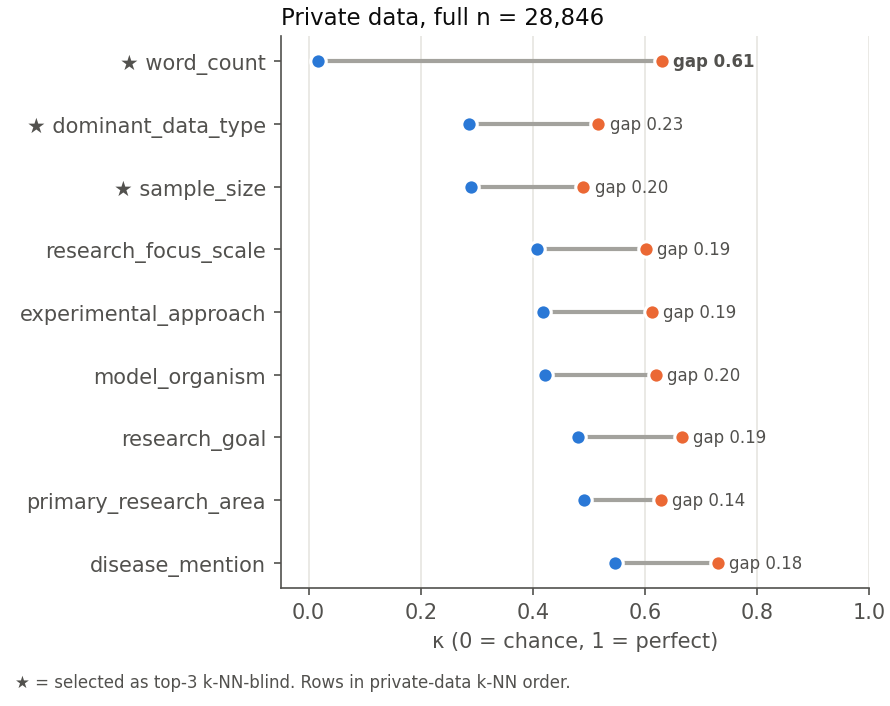
\includegraphics[width=\linewidth]{fig1_private.png}
\end{column}
\begin{column}{0.56\textwidth}
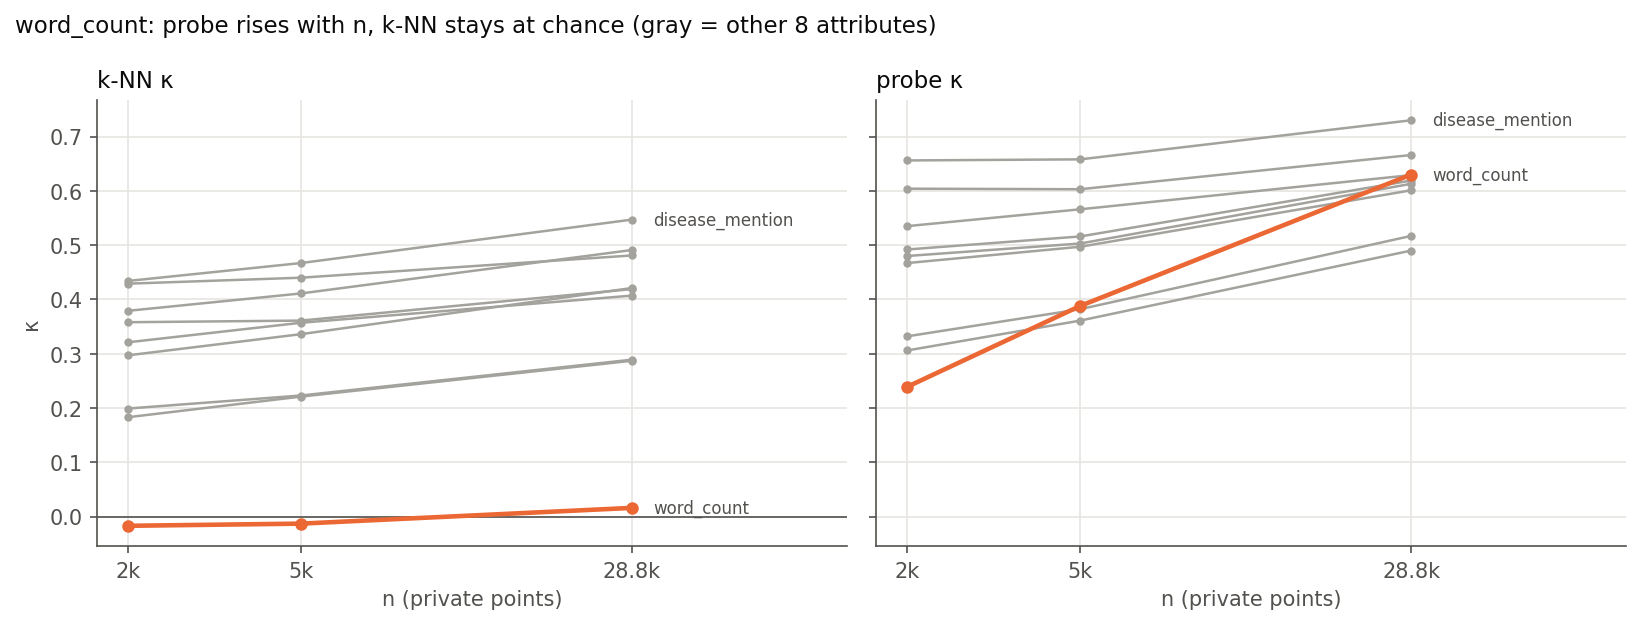
\includegraphics[width=\linewidth]{fig2_scaling_with_n.png}

\footnotesize
\begin{itemize}
  \item {\color{mut}Left: blue $\kappa^{\mathrm{NN}}$, orange $\kappa^{\mathrm{probe}}$, full $n$.}
  \item \alert{word\_count}: probe $0.24 \to 0.39 \to 0.63$ with $n$; k-NN stays $\approx 0$. Gap $0.61$, $3\times$ any other.
  \item dominant\_data\_type, sample\_size: weakly encoded (probe $\approx 0.5$, k-NN $\approx 0.29$). Other $6$: gap $0.14$--$0.23$.
  \item Top $3$ identical at all three $n$; sd $\le 0.026$.
\end{itemize}
\end{column}
\end{columns}
\end{frame}

% ------------------------------------------------------------------ 4
\begin{frame}{The blindness ranking transfers to the round-0 pool, so selection needs no private data}
\begin{columns}[T]
\begin{column}{0.40\textwidth}
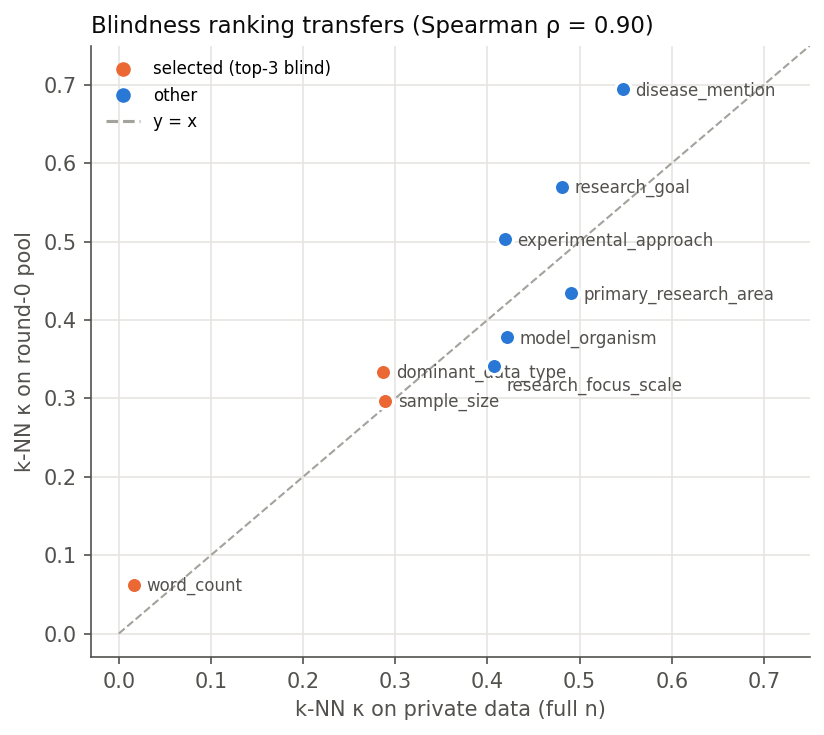
\includegraphics[width=\linewidth]{fig3_transfer_private_to_pool.png}
\end{column}
\begin{column}{0.58\textwidth}
\footnotesize
\textbf{Pool.} Qwen2.5-7B, MAPLE's prompt, AIM $\varepsilon = 4$ rows; $14{,}000$ texts saved \emph{before} the vote. Labels = requested AIM values; word\_count measured from the text.

\medskip
\textbf{Transfer.} Spearman $\rho = 0.90$ ($p = 0.001$) between private and pool $\kappa^{\mathrm{NN}}$; same top $3$ and same bottom. On the pool, $\kappa^{\mathrm{NN}}$ is \alert{post-processing} of AIM output.

\medskip
\textbf{Length compliance is poor.} Probe $\kappa$: requested length $0.22$, measured length $0.70$; $10$ length bins in the pool vs.\ $12$ requested. A length quota must use measured length.

\medskip
Most content attributes are \emph{more} visible in the pool (disease\_mention $0.69$ vs.\ $0.55$), likely because the prompt asks for every value explicitly. Same-prompt 1-NN rate is $1.3\%$, so this is not a prompt-twin effect.
\end{column}
\end{columns}
\end{frame}

% ------------------------------------------------------------------ 5
\begin{frame}{Experiment 1b: correction measures how much of the drift the real vote removes}
Run MAPLE's vote on the round-0 pool: each private point votes for its nearest pool text, Gaussian noise, keep top $K = 2000$.
For each attribute, compare three label distributions against the private target:
\[ \mathrm{correction}_k = \frac{\mathrm{JSD}_{\mathrm{random}} - \mathrm{JSD}_{\mathrm{vote}}}{\mathrm{JSD}_{\mathrm{random}} - \mathrm{JSD}_{\mathrm{floor}}}. \]
\begin{itemize}\small
  \item $\mathrm{JSD}_{\mathrm{random}}$: $K$ pool texts drawn uniformly (the generator's drift).
  \item $\mathrm{JSD}_{\mathrm{floor}}$: $K$ private texts resampled (finite-sample noise).
  \item $1$ = vote fully removes the drift, $0$ = no better than random, $<0$ = vote adds drift.
\end{itemize}
Noise $\sigma \in \{0, 2.58, 4.75, 6.87\}$, i.e.\ $\varepsilon = \infty, 4, 2, 1$ in MAPLE's schedule.

\medskip
\textbf{Which labels for the pool texts?} Requested AIM values, or labels predicted from the text by a probe trained on private Gemini labels.
\end{frame}

% ------------------------------------------------------------------ 6
\begin{frame}{Requested labels hide generator drift and make the vote look harmful}
\begin{columns}[T]
\begin{column}{0.5\textwidth}
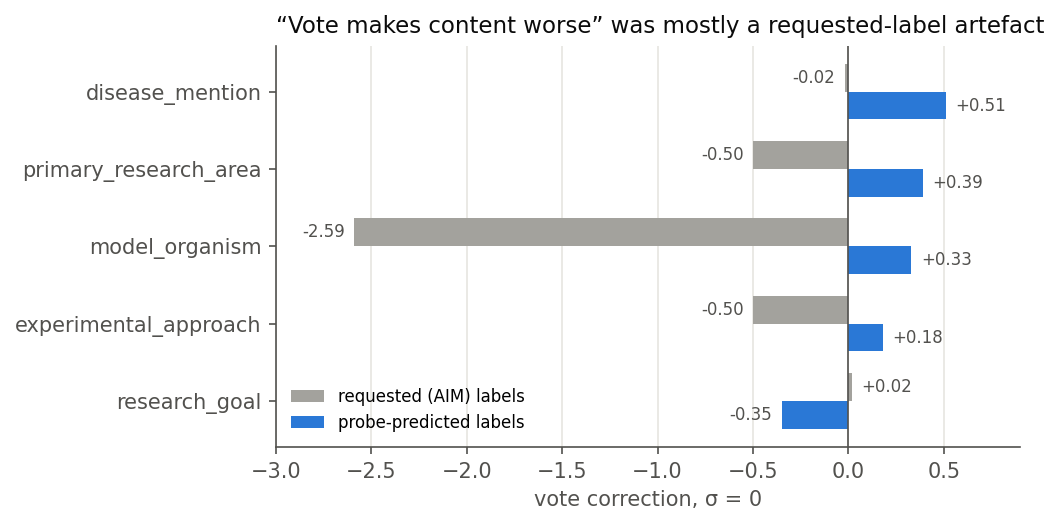
\includegraphics[width=\linewidth]{fig6_requested_vs_probe_labels.png}
\end{column}
\begin{column}{0.48\textwidth}
\small
With requested labels the vote seemed to damage content: model\_organism $-2.59$, primary\_research\_area $-0.50$.

\medskip
The vote selects texts by what they \alert{say}, but requested labels record what was \emph{asked}. The LLM follows requests only partly (compliance $\kappa$ $0.47$--$0.76$), so selected texts carry skewed requested labels even when their content improved. word\_count\_requested shows the extreme case: $-12.4$ while measured length improves by $+0.50$.

\medskip
Requested labels also match the AIM marginals by construction, so they hide the generator's drift: on probe labels, $\mathrm{JSD}_{\mathrm{random}} = 0.07$--$0.17$ vs.\ floor $\approx 0.02$--$0.04$.
\end{column}
\end{columns}
\end{frame}

% ------------------------------------------------------------------ 7
\begin{frame}{The vote corrects visible attributes; blind ones stay 4--7$\times$ above the floor}
\begin{columns}[T]
\begin{column}{0.37\textwidth}
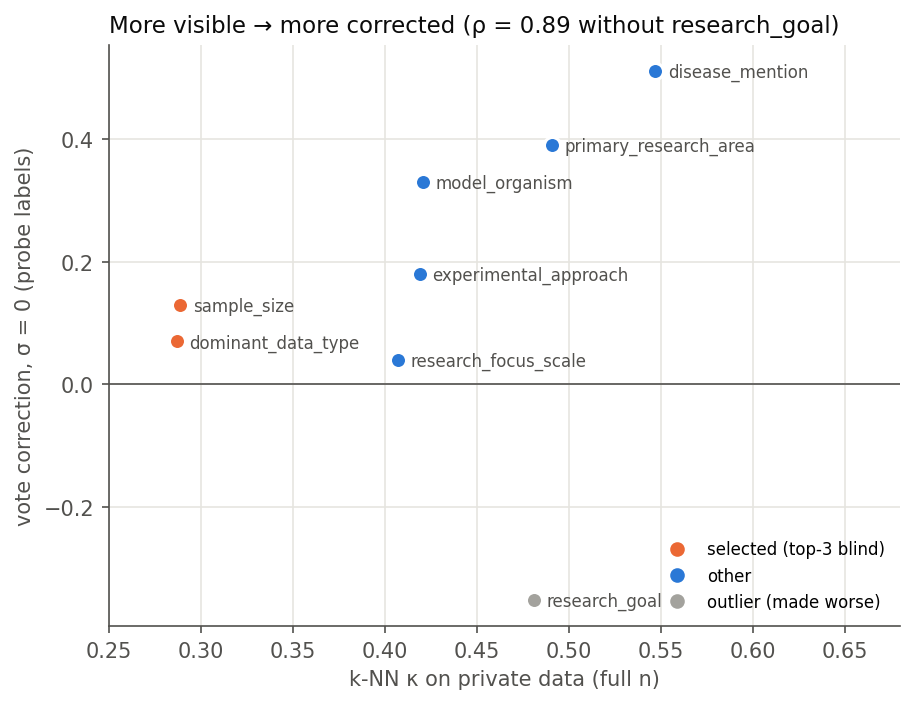
\includegraphics[width=\linewidth]{fig4_visibility_vs_correction.png}
\end{column}
\begin{column}{0.61\textwidth}
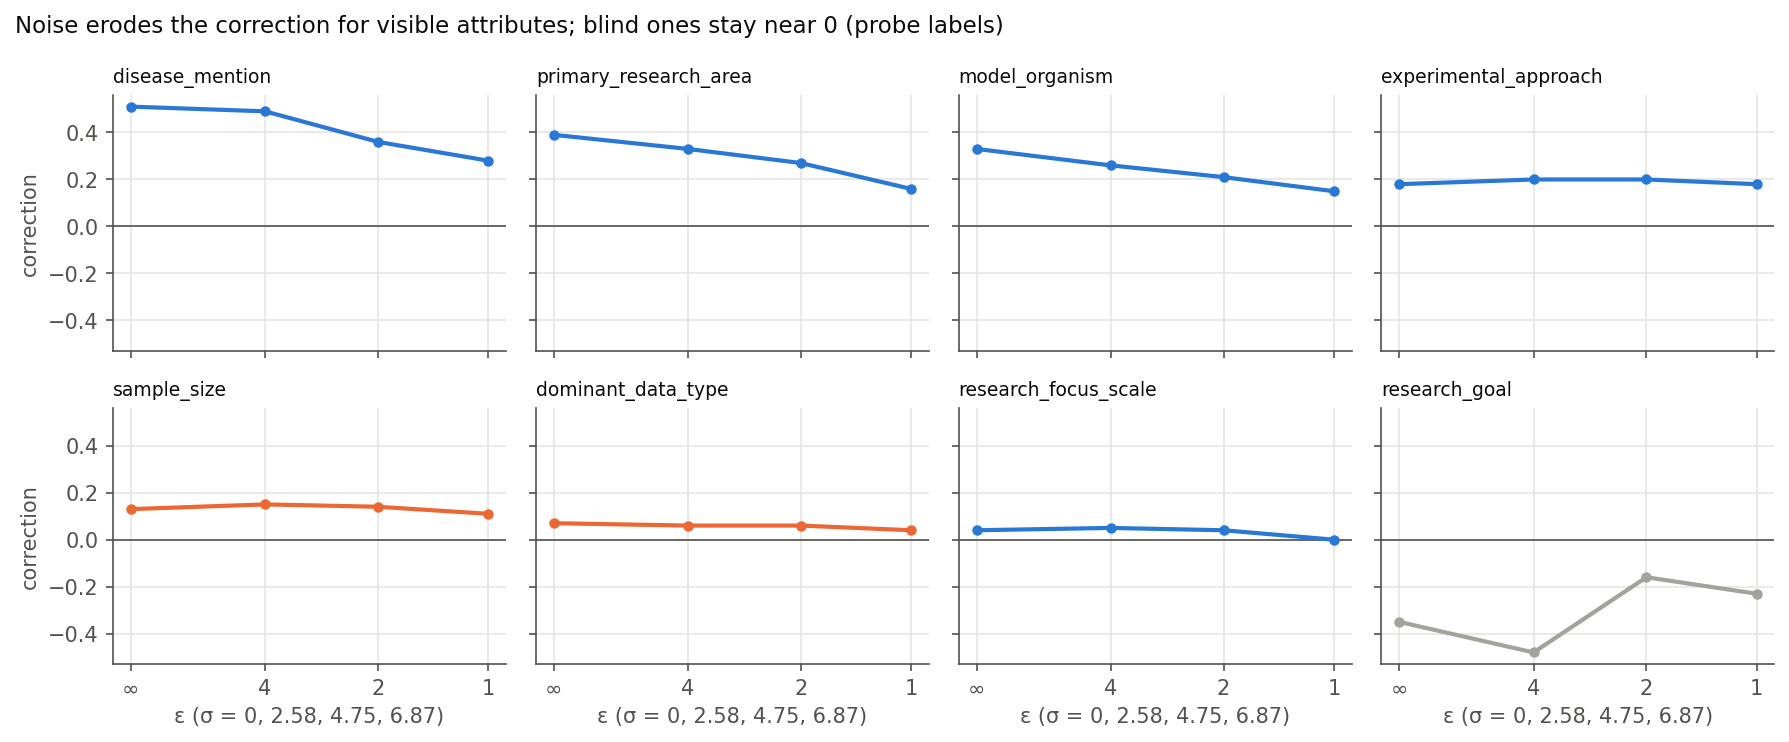
\includegraphics[width=\linewidth]{fig5_correction_vs_noise.png}
\end{column}
\end{columns}
\footnotesize
\begin{itemize}
  \item Correction at $\sigma = 0$: disease\_mention $0.51$, primary\_research\_area $0.39$, model\_organism $0.33$; sample\_size $0.13$, dominant\_data\_type $0.07$.
        Private $\kappa^{\mathrm{NN}}$ predicts it: $\rho = 0.89$ ($p = 0.007$, $7$ attributes). Outlier \alert{research\_goal}: $-0.35$ at probe $\kappa$ $0.67$.
  \item Noise erodes correction of visible attributes (disease\_mention $0.51 \to 0.28$ at $\varepsilon = 1$); blind ones stay near $0$.
\end{itemize}
\end{frame}

% ------------------------------------------------------------------ 8
\begin{frame}{Re-annotation: label once with an LLM, then classify every round cheaply}
Probe labels are circular: built on $\phi$, they see each attribute as the vote does. Testing whether the generator follows metadata needs fresh, $\phi$-independent labels in every PE round.

\medskip
\textbf{Pipeline} (\texttt{reannotate/}, set up 2026-10-11).
\begin{enumerate}\small
  \item Qwen2.5-7B annotates the $14{,}000$-text pool and $3{,}000$ private texts: MAPLE's prompt, guided JSON over the schema, greedy.
  \item Per-attribute classifiers trained on Qwen pool labels (70/15/15 split by prompt group):
        TF-IDF + LR; fine-tuned SciBERT, BiomedBERT; 2-layer MLPs (per-attribute or shared trunk + heads) on frozen $\phi$ or frozen BiomedBERT.
  \item Evaluate on pool test, private vs.\ Qwen, private vs.\ Gemini: Cohen's $\kappa$, macro-F1, marginal JSD (raw and confusion-corrected).
\end{enumerate}

\medskip
\textbf{Role split.} $\phi$-MLPs cost almost nothing, since the vote computes $\phi$ anyway: candidate \alert{quota annotator}, never the drift evaluator. The per-attribute $\kappa$ gap (best text encoder $-$ best $\phi$ model) shows whether an attribute's information is in $\phi$ at all.
\end{frame}

% ------------------------------------------------------------------ 9
\begin{frame}{Caveats and next steps}
\textbf{Caveats}
\begin{itemize}\small
  \item Length bins are ordinal but scored as nominal; both $\kappa$ values understate how much length $\phi$ sees. In 1b the vote still closes half the length gap ($\mathrm{JSD}$ $0.42 \to 0.23$, floor $0.03$).
  \item The two chance corrections differ ($\sum p^2$ vs.\ Cohen), so gaps compare only roughly across attributes.
  \item Qwen annotates its own generations; Qwen-vs-Gemini agreement on private texts bounds this.
  \item Experiment 1 on private data is a non-private diagnostic; the method uses only the pool.
\end{itemize}

\medskip
\textbf{Next}
\begin{itemize}\small
  \item Reannotate results (pending); Gemini labels for the pool once the API key arrives.
  \item Length compliance: requested vs.\ measured (MAE, histograms); length-regression probe.
  \item Experiment 2: quota on measured word\_count, sample\_size, dominant\_data\_type; JSD and MAUVE vs.\ MAPLE across $\varepsilon$.
\end{itemize}
\end{frame}

% ------------------------------------------------------------------ 10
\begin{frame}{Takeaway}
Length is encoded in $\phi$ but ignored by its $L_2$ neighbourhoods; dominant\_data\_type and sample\_size are weakly encoded. The same three attributes are selected from the privacy-free round-0 pool.

\medskip
Scored on text-derived labels, the vote corrects attributes in proportion to their k-NN visibility and leaves the blind ones uncorrected, more so under noise: the target of the quota.

\medskip
The re-annotation pipeline supplies the per-round, $\phi$-independent labels Experiment 2 needs.
\end{frame}

\end{document}
